\section{实验结果}
\label{sec:result}

\subsection*{Word Segmentation}

在训练集、开发集与测试集数据中测试结果。(表~\ref{tab:cws_result})

\begin{table}[htbp!]
    \centering
    \begin{tabular}{llccccccccc}
    \toprule
        \multicolumn{1}{c}{\multirow{2}{*}{Model}} & \multirow{2}{*}{Param}      & \multicolumn{3}{c}{Train Set}     & \multicolumn{3}{c}{Dev Set}           & \multicolumn{3}{c}{Test Set}          \\
        \multicolumn{1}{c}{}                       &                             & P             & R        & F1     & P             & R        & F1         & P             & R        & F1         \\
        \midrule
        CRF      & default                                                       & 100.00        & 100.00   & 100.00  & 100.00       & 100.00   & 100.00     & 100.00        & 100.00   & 100.00     \\
    \bottomrule
    \end{tabular}
\caption{Word segmentation (in \%)}
\label{tab:cws_result}
\end{table}

\begin{figure*}[ht]
    \begin{center}
    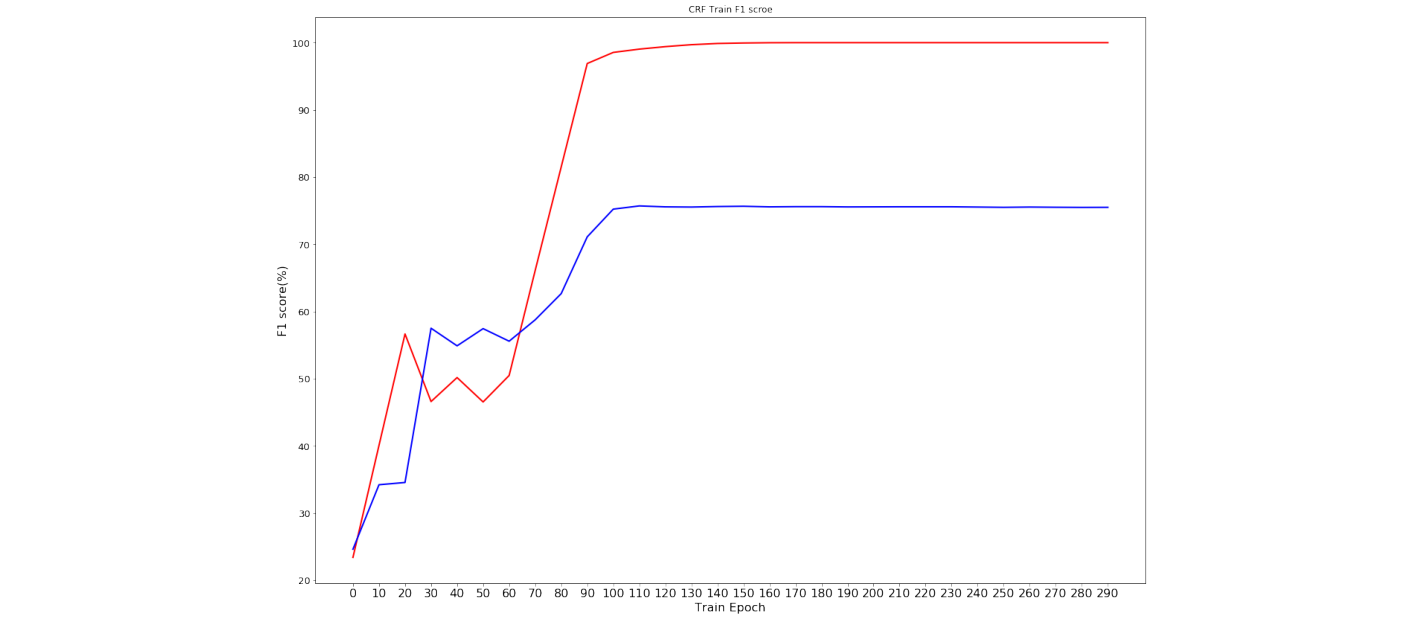
\includegraphics[width=1\textwidth]{figures/cws1.pdf}
    \end{center}
    \caption{Comparison between train epoch and the f1 score in TrainSet \& TestSet By CRF}
    \label{fig:cws1}
\end{figure*}

\begin{figure*}[ht]
    \begin{center}
    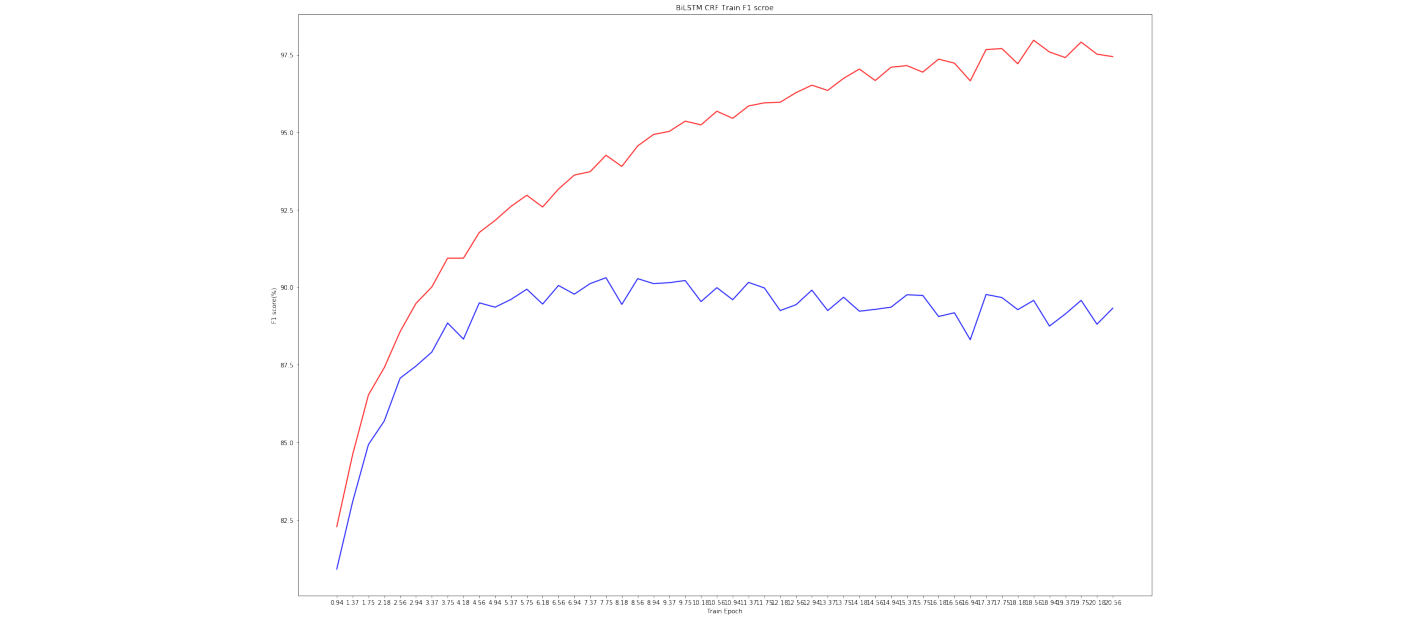
\includegraphics[width=1\textwidth]{figures/cws2.pdf}
    \end{center}
    \caption{Comparison between train epoch and the f1 score in TrainSet \& TestSet By BiLSTM-CRF}
    \label{fig:cws2}
\end{figure*}

\subsection*{Part-of-speech Tagging}

% \subsubsection*{Test on the gold word segmentation result}

在这个测试之中,排除了分词错误的可能性,利用从 testset1 中的 test\_pos1.txt 中提取出分词结果(不使用 test\_cws1.txt 是因为里面的 tag 全是乱的完全无法使用)。(表~\ref{tab:pos_on_gold_cws})

由于后面为使整体一致,补上于训练集和开发集上的评价结果,但中间状态由于并不是一个定版,故有些测试数据无法得到。

关于这些数据可以观察到几点,首先 precision、recall、f1-score 值在此项测试中会相等的原因在词性标注的实验原理中~\ref{sec:pos}已经叙述过了。再来是训练集并不因规则而有所提升,这也很容易想,因为由于我们是从训练集建立的关联关系,故训练集并不会存在 OOV 的问题,故提升上只会在开发集和测试集中体现。

\begin{table}[htbp!]
    \centering
    \begin{tabular}{lccc}
    \toprule
        Method          & F1-Score on Train Set  & F1-Score on Dev Set   & F1-Score on Test Set \\
    \midrule
        Pure Mapping    & 97.98                  & 95.57                 & 95.39                \\
        Add Rules       & -                      & -                     & 95.83                \\
        Even More Rules & 97.98                  & 96.06                 & 95.86                \\
    \bottomrule
    \end{tabular}
\caption{Part-of-speech tagging on Gold CWS (in \%) (precision = recall = f1-score)}
\label{tab:pos_on_gold_cws}
\end{table}

% \subsection*{Overall Test}

% 将所有测试文档还原成原始文档进行分析的结果。(表~\ref{tab:pos_with_cws})

% \begin{table}[htbp!]
    \centering
    \begin{tabular}{llccccccccc}
    \toprule
        \multicolumn{2}{c}{Experiment}    & \multicolumn{3}{c}{Train Set}  & \multicolumn{3}{c}{Dev Set} & \multicolumn{3}{c}{Test Set}  \\
        CWS Method      & POS Method      & P     & R     & F1             & P     & R     & F1          & P     & R     & F1            \\
    \midrule
        CRF             & With Rule       & 95.39 & 95.39 & 95.39          & 95.39 & 95.39 & 95.39       & 95.39 & 95.39 & 95.39         \\
    \bottomrule
    \end{tabular}
\caption{Entire process result from raw article to evaluation (in \%)}
\label{tab:pos_with_cws}
\end{table}
